\section{Object Recognition}
To be able to figure out where the target is, its location within the video stream has to be determined.
It is not enough to simply answer the binary question "is a target present?" but rather "where is the target located?", so this information can be processed and in turn move the motors to point the laser at the target.
As mentioned in section~\ref{sec:obj_tracking}, object recognition algorithms can be tedious to do by hand, and as a result of this, machine learning algorithms will be utilized.
Although the initial target of the device may be a simple and easily recognizable object, the intent is to create a solution that can identify more complex targets, in a potentially noisy environment.
Because of this, it is important to look into the science of object identification, what algorithms and methods exists, and what libraries we have at our disposal.

\subsection{Neural Networks}

A neural network is, as the name implies, a network of neurons.
It is based on neuroscience, especially the inner workings of the human brain, where a network of neurons is used to make decisions.
The difference being, whether it is a biological neural network or an artificial one, which is the case in a computer science context.
In computer science, a neuron can be seen as a function, that processes some input and then transmits the processed value to connected neurons \cite{ANN}.

Neural networks are a powerful but complex method of doing machine learning.
Because of this, simpler solutions should also be considered when exploring which methods suits the task best.
One of the reasons neural networks are especially interesting in this case, is its ability to recognize patterns \cite{ANN}.
Pattern recognition is a fundamental part of object recognition making neural networks an obvious option.


\subsubsection{Convolutional Neural Network}
Convolutional neural networks (CNN) are often used for image classification, and is the most popular type of neural network in regards to object detection\cite{CNN}.
In challenges such as LSVCR\footnote{Imagenet Large Scale Visual Recognition Challenge} the majority of the entries are done using CNN \cite{ILSVRC_Results}.  
A CNN is a neural network in which neurons are grouped into layers.
These layers are grouped in three categories; an input layer, an output layer and a number of so called hidden layers.
The goal of the hidden layers are to transform the input data into the expected output data.
It does this by doing abstractions within each layer, breaking a complex problem into smaller, more trivial, sub-problems.

In terms of object recognition, an example could be face recognition.
The first layer could recognize lines, edges or similar low level features.
The following layers could then detect increasingly complicated facial features, ending at some layer, in which one neuron would transmit a signal if a nose is present in the image, and another neuron to transmit if a mouth is present.


\begin{figure}[H]
	\centering
	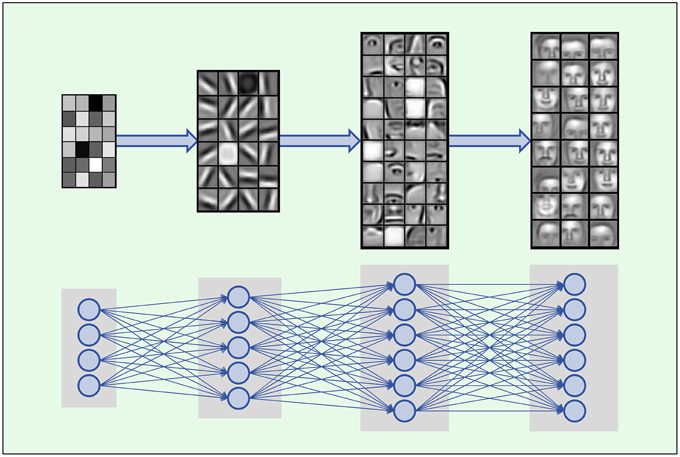
\includegraphics[scale=0.40]{images/cnn_face.jpg}
	\caption{A simplified example of the abstractions within a CNN.}
	\label{fig:face_cnn}
	\cite{CNNStructure}
\end{figure}
 
However, it is important to understand, that this is not necessarily the patterns that a CNN will detect within its layers.
Actually it is far more likely, that the layers will recognize something that to a human has no relation to a face.
But the computer will have found a correlation between these seemingly random patterns, and a face.

CNNs are often used along with pooling \cite{CNN}.
Pooling is a concept in which multiple outputs are combined into a single neuron in the next layer.
This can be done in order to down-sample the input and reduce the complexity making the CNN run faster.
Some common examples of pooling is max pooling and average pooling, in which the average or max value is output from a number of input neurons.

CNNs are an effective choice for classification. 
This means it can answer yes or no to whether the image is of a car.
Now the question is whether it can be used to figure out the position of the objects within the image.
The answer turns out to be yes.


\subsubsection{Regional Convolutional Neural Network}

A regional convolutional neural network (RCNN) utilizes CNN to get both a classification along with a bounding box, which in turn can be used to determine the center of the location.
It does this by applying the CNN to smaller regions of the image. 
These regions are extracted from the image using a method called selective search.
If the region contains an element recognized by the CNN a bounding box can be drawn around the region.
The bounding box can at last be tightened using different methods, a popular option being a linear regression model.\cite{CNNHistory}

Unfortunately RCNN in itself is not viable for real time object detection.
However, there have been a lot of modifications and improvements of RCNN that improves the performance of it.
One improvement is called fast RCNN and is leaning toward being feasible for real time object detection.

%\subsection{You Only Look Once}

%An alternative to RCNN is You Only Look Once (YOLO) which is a new technology developed with real time processing in mind.



\subsection{GOTURN}
% https://www.learnopencv.com/goturn-deep-learning-based-object-tracking/
Generic Object Tracking Using Regression Networks, is an algorithm based on deep learning\cite{goturn}.
GOTURN is different than the majority of algorithms presented in this section, in that it uses offline learning, whereas online learning constantly improves the model during run-time.
It utilizes a large test set of videos of different objects and is taught with the help of this.
The model is then shipped with the algorithm implementation.
The benefit of this, is that it runs faster, as it does not have to ever modify the model or analyze whether the given result is relevant.
However, this comes at a cost. 
The algorithm has a tendency to favor objects within the training set, even if they remain stationary.
So, for instance, if we want to track a bird flying past stationary planes, it might lock onto the planes rather than the bird, even though the planes are not moving.
This is due to the unpredictability of what the algorithm see as a correlation between video and a correct answer.


The GOTURN algorithm utilizes CNN, which is explained in the previous sub-section.
\begin{figure}[H]
	\centering
	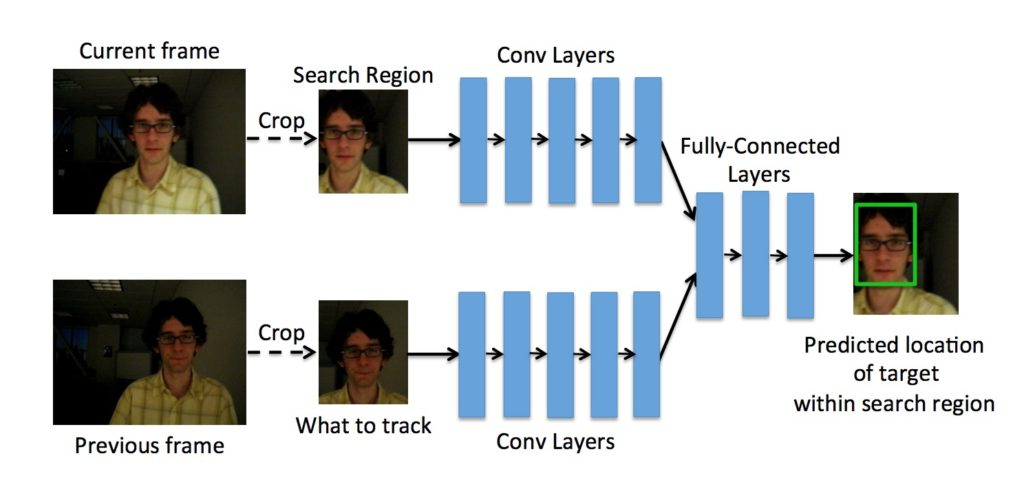
\includegraphics[scale=0.80]{images/GOTURN-architecture.jpg}
	\caption{How the algorithm utilizes CNN \cite{goturn}.}
	\label{fig:goturn-arch}
\end{figure}
GOTURN works by looking at two frames the first, also known as previous frame, and the second, also known as current frame.
This is also shown on Figure~\ref{fig:goturn-arch}.
The premise is that the location of the object is known in previous frame, and a bounding box is present.
Based on the bounding box of the previous frame, the current frame is cropped to two times the size of the previous bounding box.
A CNN is then trained to predict the bounding box in the second frame.


Some possible problems with this algorithm is that the location of the target is not known initially, as the target will not necessarily be in the picture at startup time, and will eventually leave the image feed again, as our device will have idle time.
Another possible issue would be depending on the speed of the given target and the frame-rate of the camera, as the object might have left the cropped area. 
This could be solved by a larger crop, however this makes it less relevant.

\subsection{OpenCV}
One option is to simply utilize the highly popular OpenCV library.
OpenCV is an open source computer vision library, that comes with ready to use object tracking functionality.
% Write more



\subsection{Tensorflow}
%Tensorflow is a python framework for working with machine learning.
%It is beginner friendly but still has the possibilities of delving deeper into the inner workings of a given model, and the processes of it.



% https://github.com/tensorflow/models/tree/master/research/object_detection

% Mine noter af ting at skrive
	% what is a tensor
	% training
	% exporting from it
	% can be used with any alogrithm 
	% hvorfor er det så nice at arbejde med
	% hvordan kan vi få brug af dette


% Things to check / consider writing about
% https://en.wikipedia.org/wiki/Computer_vision#Recognition
% https://en.wikipedia.org/wiki/Video_tracking
% Kernel-based tracking
% Contour tracking
% https://en.wikipedia.org/wiki/Kalman_filter
% Particle filter
% https://en.wikipedia.org/wiki/Outline_of_object_recognition
% real-time: triangulate each frame and measure the persistence of selected triangles relative to their location in each successive frame. 
% Microprocessors such as the raspberry pi are fast enough so that triangulation and triangle measurement can be done in a few milliseconds.
% ^^ Few miliseconds (Sounds like maybe around 5ms, would alow for updating robot position 20 times a second (capture 20 fps from the camera too). 
% Which could be a goal to aim at (RTS: scheduling bla bla, update canon position 20 times pr second...))
% Would be cool in RTS part to integrate some functionality to handle if camera data is not ready within the 5 ms, or if the device is not ready to handle input after 5 ms. 
% The MI part could be coded to update each 5 ms.
